\chapter*{Appendix}
\renewcommand{\thesection}{\Alph{section}}
\section{Pre-activation Pattern} \label{app:feature_bias}

This section presents the gradient distance graph $\mathcal{B}^{(ci)}_{gr}$ for the feature-based model. Section \ref{sec:cav_extraction} discussed that the activation $\boldsymbol{h}$ for extracting CAV is the hidden layer output after the activation function, with the $\mathcal{B}^{(ci)}_{gr}$ graph in Figure \ref{fig:post-activation}. An experiment is attempted to extract CAVs using pre-activation values, which are the hidden layer outputs before the activation function, with the $\mathcal{B}^{(ci)}_{gr}$ graph in Figure \ref{fig:pre-activation}.

\begin{figure}[H]
    \centering
    \begin{minipage}[t]{0.48\textwidth}
        \centering
        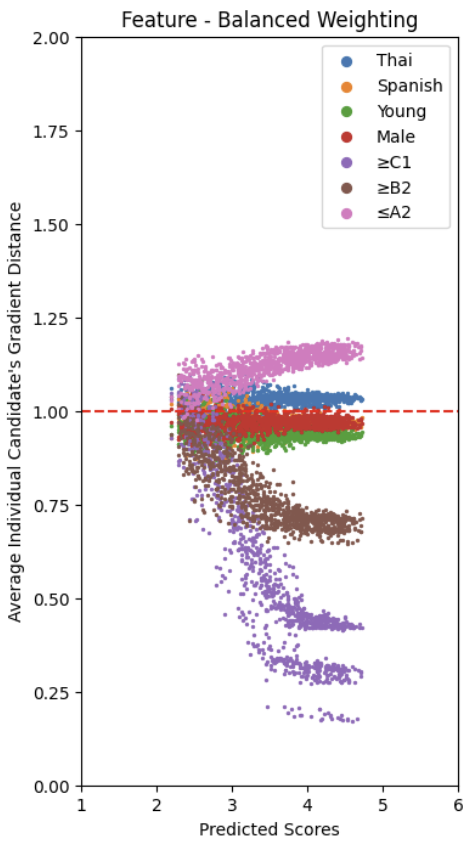
\includegraphics[width=0.4\linewidth]{feature_balanced.png}
        \caption{$\mathcal{B}^{(ci)}_{gr}$ for the feature-based model using post-activation values for CAV extraction}
        \label{fig:post-activation}
    \end{minipage}
    \hfill
    \begin{minipage}[t]{0.48\textwidth}
        \centering
        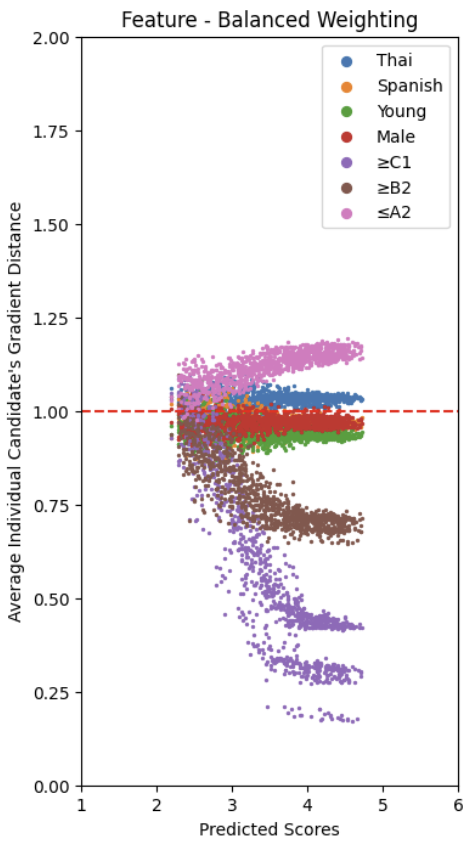
\includegraphics[width=0.4\linewidth]{feature_balanced_old.png}
        \caption{$\mathcal{B}^{(ci)}_{gr}$ for the feature-based model using pre-activation values for CAV extraction}
        \label{fig:pre-activation}
    \end{minipage}
\end{figure}

The pre-activation graph has a thick, fan-shaped pattern, which is more similar to the pattern in Xizi's paper \cite{feature_bias}. The paper's auto marker grader used LReLU activation function, which should have the effect of narrowing the lines in the graph to patterns similar to Figure \ref{fig:post-activation}. This therefore suggests a possibility that the activation $\boldsymbol{h}$ in \cite{feature_bias} might be extracted from the pre-activation values instead.

\section{Risk Assessment}
This appendix outlines the project's risk assessment. Key risks included repetitive strain injury (RSI), eye strain, and hazards like tripping over cables or burns from overheated components. Mitigation measures included:

\begin{itemize}
    \item Scheduling regular breaks to reduce typing strain.
    \item Adjusting desk and screen height to maintain ergonomic posture.
\end{itemize}
